\documentclass[conference]{IEEEtran}
% \IEEEoverridecommandlockouts
% The preceding line is only needed to identify funding in the first footnote. If that is unneeded, please comment it out.
% Template version as of 6/27/2024

\usepackage{cite}
\usepackage{amsmath,amssymb,amsfonts}
\usepackage{algorithmic}
\usepackage{graphicx}
\usepackage{textcomp}
\usepackage{xcolor}
\usepackage{tikz}

\usetikzlibrary{automata, positioning}
\tikzset{
->, % makes the edges directed
>=stealth, % makes the arrow heads bold
node distance=1.7cm, % specifies the minimum distance between two nodes. Change if necessary.
every state/.style={thick}, % sets the properties for each ’state’ node
initial text=$ $, % sets the text that appears on the start arrow
}

\def\BibTeX{{\rm B\kern-.05em{\sc i\kern-.025em b}\kern-.08em
    T\kern-.1667em\lower.7ex\hbox{E}\kern-.125emX}}
\graphicspath{
    {img/}
}

\begin{document}

\title{An Implementation of Product Construction on Deterministic Finite Automata in Python}

\author{
\IEEEauthorblockN{Evan Childers}
\IEEEauthorblockA{
\textit{University of Alabama}\\
Tuscaloosa, Alabama, United States \\
epchilders@crimson.ua.edu}
\and
\IEEEauthorblockN{August Connors}
\IEEEauthorblockA{
\textit{University of Alabama}\\
Tuscaloosa, Alabama, United States \\
ahconnors@crimson.ua.edu}
\and
\IEEEauthorblockN{Kai NeSmith}
\IEEEauthorblockA{
\textit{University of Alabama}\\
Tuscaloosa, Alabama, United States \\
klnesmith@crimson.ua.edu}
}

\maketitle

\begin{abstract}
ABSTRACT HERE - ALL
\end{abstract}

\section{Introduction}
In automata theory, product construction describes the method by which two deterministic finite automata (DFAs) are combined into a single DFA to accept a language that is derived from a certain boolean operation on the languages of the original DFA's such as intersection and union. This method plays a pivotal role in many applications in computing theory and formal language processing. In particular, product construction provides a means for which relationships between regular languages can be explored. By constructing a product DFA, one can effectively evaluate whether two DFAs accept overlapping inputs, meet certain logical requirements, or satisfy a desired system behavior.

\section{Problem Statement}
While the process of DFA product construction is a well understood concept in automata theory, the manual computation of a product DFA can become extremely complex and error-prone as the size of the DFAs involved increase. Additionally, the intricacy of these product DFAs can often complicate the process of verifying logical operations like the intersection and union of different automata. This sparks the need for a programmatic solution capable of systematically identifying the product states and transitions, simulating the traversal of a DFA given an input string and presenting the resulting automaton in a clear and interpretable form. This work addresses the lack of available resources regarding this issue by detailing the implementation and formal proof for product construction in Python, along with its potential use cases in verifying logical expressions.

\section{Implementation}
\textbf{IMPLEMENTATION DETAILS HERE - AUGIE}

\section{Experiments}
In this section, we will explore how product construction can be applied to a variety of different DFA's with a focus on the differences between intersection and union as well as identifying the causes of unreachable states in the resulting automaton

\subsection{Experiment 1}
In this experiment, we started with two DFAs to product construct in order to test the basic capabilities of our implementation. The first DFA, whose transition table is shown in Table \ref{table-exp1-dfa1} and diagram shown in Fig. \ref{fig-exp1-dfa1}, accepts the language that contains strings of length at least two that have a 1 in their second position.

\begin{table}[h!]
    \caption{Experiment 1's DFA 1 Transition Table}
    \begin{displaymath}
        \begin{array}{r|c|c|}
        & 0 & 1 \\
        \hline
        \rightarrow a_0 & a_1 & a_1 \\
        a_1 & a_r & a_2 \\
        * a_2 & a_2 & a_2 \\
        a_r & a_r & a_r \\
        \end{array}
    \end{displaymath}
    \label{table-exp1-dfa1}
\end{table}
\begin{figure}[h!]
    \centering
    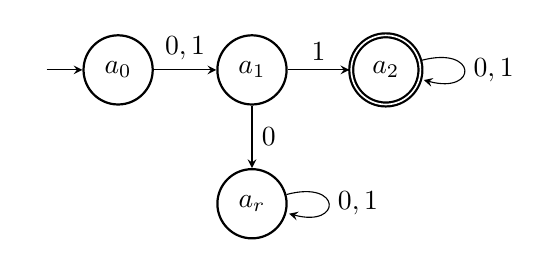
\begin{tikzpicture}
        \node[state, initial] (a0) {$a_{0}$};
        \node[state, right of=a0] (a1) {$a_{1}$};
        \node[state, right of=a1, accepting] (a2) {$a_{2}$};
        \node[state, below of=a1] (areject) {$a_{r}$};
    
        \draw (a0) edge[above] node{$0,1$} (a1)
              (a1) edge[above] node{$1$} (a2)
                   edge[right] node{$0$} (areject)
              (a2) edge[loop right] node{$0,1$} (a2)
              (areject) edge[loop right] node{$0,1$} (areject);
    \end{tikzpicture}
    \caption{Experiment 1's DFA 1}
    \label{fig-exp1-dfa1}
\end{figure}

The second DFA, whose transition table is shown in Table \ref{table-exp1-dfa2} and diagram shown in Fig. \ref{fig-exp1-dfa2}, accepts the language that contains strings that contain at least one 0.

\begin{table}[h!]
    \caption{Experiment 1's DFA 2 Transition Table}
    \begin{displaymath}
        \begin{array}{r|c|c|}
        & 0 & 1 \\
        \hline
        \rightarrow b_0 & b_1 & b_0 \\
        * b_1 & b_1 & b_1 \\
        \end{array}
    \end{displaymath}
    \label{table-exp1-dfa2}
\end{table}
\begin{figure}[h!]
    \centering
    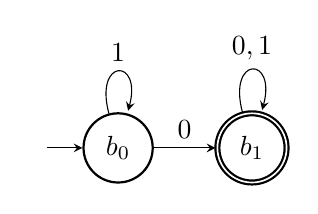
\begin{tikzpicture}
        \node[state, initial] (b0) {$b_{0}$};
        \node[state, right of=b0, accepting] (b1) {$b_{1}$};

        \draw (b0) edge[above] node{$0$} (b1)
                   edge[loop above] node{$1$} (b0)
              (b1) edge[loop above] node{$0,1$} (b1);
    \end{tikzpicture}
    \caption{Experiment 1's DFA 2}
    \label{fig-exp1-dfa2}
\end{figure}

When computing the product of these two DFA's, the resulting transition table is:

\begin{table}[h!]
    \caption{Experiment 1's Product DFA Transition Table}
    \begin{displaymath}
        \begin{array}{r|c|c|}
        & 0 & 1 \\
        \hline
        \rightarrow a_0,b_0 & a_1,b_1 & a_1,b_0 \\
        a_0,b_1 & a_1,b_1 & a_1,b_1 \\
        a_1,b_0 & a_r,b_1 & a_2,b_0 \\
        a_1,b_1 & a_r,b_1 & a_2,b_1 \\
        a_2,b_0 & a_2,b_1 & a_2,b_0 \\
        * a_2,b_1 & a_2,b_1 & a_2,b_1 \\
        a_r,b_0 & a_r,b_1 & a_r,b_0 \\
        a_r,b_1 & a_r,b_1 & a_r,b_1 \\
        \end{array}
    \end{displaymath}
    \label{table-exp1-dfaprod}
\end{table}

The algorithmically determined unreachable states are \( (a_0, b_1) \) and \( (a_r, b_0) \). When analyzing these state pairs in the context of their original DFAs, we can understand why they are unreachable in the product DFA. For the state pair \( (a_0, b_1) \), note that \( b_1 \) can only be reached from DFA 2’s start state by a transition on input 0. However, in DFA 1, \( a_0 \) transitions to a different state on input 0 and does not allow any transitions that lead back to \( a_0 \). Therefore, there is no string that leads to the simultaneous presence of \( a_0 \) and \( b_1 \), rendering this state pair unreachable in the product. A similar rationale applies to \( (a_r, b_0) \). The state \( a_r \) in DFA 1 is reached via a transition on input 0, while \( b_0 \) in DFA 2 transitions away from itself on input 0 and does not return. Thus, there is no string in the input alphabet that can result in the system being in the state \( (a_r, b_0) \), making it unreachable as well. \\


In order to verify the intersection and union properties, we use the \texttt{accepts\_string} method to test string acceptance in the product DFA. The results demonstrate the logical operations between the original DFAs:

\begin{table}[h!]
\centering
\caption{Boolean Analysis of Product DFA Operations}
\label{table-dfa_boolean}
\begin{tabular}{|c|c|c|c|c|}
\hline
\textbf{DFA Type} & \textbf{11} & \textbf{00} & \textbf{01} & \textbf{1} \\ \hline
DFA 1 & True & False & True & False \\ \hline
DFA 2 & False & True & True & False \\ \hline
Union DFA & True & True & True & False \\ \hline
Intersection DFA & False & False & True & False \\ \hline
\end{tabular}
\end{table} 

As shown in table, the union DFA accepts a string if either original DFA accepts it ($\text{DFA}_1 \cup \text{DFA}_2$), while the intersection DFA only accepts strings accepted by both ($\text{DFA}_1 \cap \text{DFA}_2$). The results confirm the correct implementation of these Boolean operations.


\subsection{Experiment 2}


\textbf{EXPERIMENTS HERE - EVAN \& KAI}

\section{Contributions}
\subsection{Evan Childers}
\textbf{EVAN CONTRIBUTIONS HERE}
\subsection{August Connors}
\textbf{AUGIE CONTRIBUTIONS HERE}
\subsection{Kai NeSmith}
\textbf{KAI CONTRIBUTIONS HERE}

\section{Conclusion}
\textbf{CONCLUSION HER - KAI (ALL)}

% Not sure if we'll need a bibliography, so leaving the template here in case.
\begin{thebibliography}{00}
\bibitem{b1} G. Eason, B. Noble, and I. N. Sneddon, ``On certain integrals of Lipschitz-Hankel type involving products of Bessel functions,'' Phil. Trans. Roy. Soc. London, vol. A247, pp. 529--551, April 1955.
\end{thebibliography}

\end{document}
